\documentclass[11pt,a4paper]{article}
\usepackage[margin=1in]{geometry}
\usepackage[T1]{fontenc}
\usepackage[utf8]{inputenc}
\usepackage{lmodern,amsmath,amssymb,booktabs,graphicx,microtype}
\usepackage[hidelinks]{hyperref}
\usepackage{url}
\setlength{\parskip}{0.35em}
\setlength{\parindent}{0pt}
\setlength{\emergencystretch}{2em}
% Generated from results/aggregate_results.json. Do not hand-edit.
\newcommand{\BaselineFone}{0.8534}
\newcommand{\BaselineAccuracy}{0.8714}
\newcommand{\BaselineRecall}{0.8063}
\newcommand{\BaselineSpecificity}{0.9023}
\newcommand{\BaselineFeatures}{288}
\newcommand{\BaselineReduction}{0.00}
\newcommand{\FuzzyFone}{0.8501}
\newcommand{\FuzzyAccuracy}{0.8673}
\newcommand{\FuzzyRecall}{0.8196}
\newcommand{\FuzzySpecificity}{0.8901}
\newcommand{\FuzzyFeatures}{7.6}
\newcommand{\FuzzyReduction}{97.36}
\newcommand{\GBFone}{0.8540}
\newcommand{\GBAccuracy}{0.8726}
\newcommand{\GBRecall}{0.8030}
\newcommand{\GBSpecificity}{0.9060}
\newcommand{\GBFeatures}{13}
\newcommand{\GBReduction}{95.49}
\newcommand{\PrimaryTable}{%
\begin{tabular}{lrrrr}\toprule
Method & Macro-F1 & Accuracy & Features & Reduction (\%)\\\midrule
All features & 0.8534 $\pm$ 0.0436 & 0.8714 $\pm$ 0.0389 & 288 & 0.00 \\
Fuzzy-rough & 0.8501 $\pm$ 0.0362 & 0.8673 $\pm$ 0.0312 & 7.6 & 97.36 \\
GBFRS reconstruction & 0.8540 $\pm$ 0.0417 & 0.8726 $\pm$ 0.0346 & 13 & 95.49 \\
\bottomrule\end{tabular}}
\newcommand{\ClinicalTable}{%
\begin{tabular}{lrrr}\toprule
Method & Balanced accuracy & Malignant recall & Benign specificity\\\midrule
All features & 0.8543 $\pm$ 0.0454 & 0.8063 $\pm$ 0.0748 & 0.9023 $\pm$ 0.0377 \\
Fuzzy-rough & 0.8548 $\pm$ 0.0395 & 0.8196 $\pm$ 0.0643 & 0.8901 $\pm$ 0.0178 \\
GBFRS reconstruction & 0.8545 $\pm$ 0.0465 & 0.8030 $\pm$ 0.0841 & 0.9060 $\pm$ 0.0200 \\
\bottomrule\end{tabular}}
\newcommand{\StabilityTable}{%
\begin{tabular}{lrrr}\toprule
Method & Mean Jaccard & Nogueira stability & Total time (s)\\\midrule
All features & 1.000 & 1.000 & 177.0 \\
Fuzzy-rough & 0.249 & 0.378 & 33.0 \\
GBFRS reconstruction & 0.531 & 0.678 & 211.2 \\
\bottomrule\end{tabular}}
\newcommand{\EffectTable}{%
\begin{tabular}{lrr}\toprule
Comparison & Pooled macro-F1 difference & 95\% interval\\\midrule
Fuzzy-rough minus All features & -0.0034 & [-0.0188, +0.0118] \\
GBFRS reconstruction minus All features & +0.0008 & [-0.0122, +0.0139] \\
GBFRS reconstruction minus Fuzzy-rough & +0.0042 & [-0.0069, +0.0158] \\
\bottomrule\end{tabular}}

% Generated from validated aggregate-only secondary results.
\newcommand{\BusSecondaryTable}{%
\begin{tabular}{lrrr}
\toprule
Method & Macro-F1 (mean $\pm$ SD) & Accuracy & Features \\
\midrule
All-feature SVM & 0.8534 $\pm$ 0.0436 & 0.8714 & 288.0 \\
Fuzzy-rough + SVM & 0.8501 $\pm$ 0.0362 & 0.8673 & 7.6 \\
GBFRS reconstruction + SVM & 0.8540 $\pm$ 0.0417 & 0.8726 & 13.0 \\
ANOVA + SVM & 0.8391 $\pm$ 0.0420 & 0.8592 & 11.0 \\
Mutual information + SVM & 0.8469 $\pm$ 0.0488 & 0.8668 & 9.0 \\
L1 logistic selection + SVM & 0.8447 $\pm$ 0.0323 & 0.8620 & 30.8 \\
Unchanged author selector + SVM & 0.5034 $\pm$ 0.0396 & 0.5730 & 1.8 \\
\bottomrule
\end{tabular}}

\newcommand{\WdbcTable}{%
\begin{tabular}{lrrr}
\toprule
Method & Macro-F1 (mean $\pm$ SD) & Accuracy & Features \\
\midrule
All-feature SVM & 0.9772 $\pm$ 0.0265 & 0.9789 & 30.0 \\
Fuzzy-rough + SVM & 0.9455 $\pm$ 0.0171 & 0.9491 & 5.6 \\
GBFRS reconstruction + SVM & 0.9603 $\pm$ 0.0217 & 0.9631 & 4.8 \\
ANOVA + SVM & 0.9772 $\pm$ 0.0161 & 0.9789 & 20.0 \\
Mutual information + SVM & 0.9720 $\pm$ 0.0114 & 0.9737 & 20.0 \\
L1 logistic selection + SVM & 0.9680 $\pm$ 0.0142 & 0.9702 & 14.2 \\
Unchanged author selector + SVM & 0.8366 $\pm$ 0.0974 & 0.8452 & 2.8 \\
\bottomrule
\end{tabular}}

% Generated from validated aggregate-only records.

\newcommand{\NoiseTable}{%
\begin{tabular}{lrrr}
\toprule
Setting & Macro-F1 (mean $\pm$ SD) & Accuracy & Features \\
\midrule
All-feature SVM: 0\% & 0.8534 $\pm$ 0.0436 & 0.8714 & 288.0 \\
All-feature SVM: 10\% & 0.8299 $\pm$ 0.0359 & 0.8512 & 288.0 \\
All-feature SVM: 20\% & 0.8094 $\pm$ 0.0421 & 0.8373 & 288.0 \\
Fuzzy-rough + SVM: 0\% & 0.8501 $\pm$ 0.0362 & 0.8673 & 7.6 \\
Fuzzy-rough + SVM: 10\% & 0.7898 $\pm$ 0.0699 & 0.8095 & 7.8 \\
Fuzzy-rough + SVM: 20\% & 0.7548 $\pm$ 0.0583 & 0.7726 & 8.2 \\
GBFRS reconstruction + SVM: 0\% & 0.8540 $\pm$ 0.0417 & 0.8726 & 13.0 \\
GBFRS reconstruction + SVM: 10\% & 0.8405 $\pm$ 0.0380 & 0.8609 & 16.6 \\
GBFRS reconstruction + SVM: 20\% & 0.8181 $\pm$ 0.0414 & 0.8401 & 17.6 \\
\bottomrule
\end{tabular}}

\newcommand{\SensitivityTable}{%
\begin{tabular}{lrrr}
\toprule
Setting & Macro-F1 (mean $\pm$ SD) & Accuracy & Features \\
\midrule
Own: purity 0.90, seed 42 & 0.8540 $\pm$ 0.0417 & 0.8726 & 13.0 \\
Own: purity 0.80, seed 42 & 0.8537 $\pm$ 0.0351 & 0.8705 & 14.8 \\
Own: purity 0.95, seed 42 & 0.8525 $\pm$ 0.0392 & 0.8699 & 12.8 \\
Own: purity 0.90, seed 43 & 0.8525 $\pm$ 0.0312 & 0.8706 & 14.2 \\
Own: purity 0.90, seed 44 & 0.8504 $\pm$ 0.0393 & 0.8684 & 14.6 \\
Alternative criterion: same balls & 0.5051 $\pm$ 0.0393 & 0.5746 & 1.8 \\
\bottomrule
\end{tabular}}

\newcommand{\ExternalTable}{%
\begin{tabular}{lrrr}
\toprule
Setting & Macro-F1 (mean $\pm$ SD) & Accuracy & Features \\
\midrule
All-feature SVM & 0.6886 $\pm$ 0.0545 & 0.7022 & 102.0 \\
Fuzzy-rough + SVM & 0.6737 $\pm$ 0.0359 & 0.6944 & 5.8 \\
GBFRS reconstruction + SVM & 0.6700 $\pm$ 0.0580 & 0.6865 & 12.2 \\
ANOVA + SVM & 0.7296 $\pm$ 0.0623 & 0.7460 & 18.0 \\
Mutual information + SVM & 0.7172 $\pm$ 0.0429 & 0.7302 & 18.0 \\
L1 logistic selection + SVM & 0.7272 $\pm$ 0.0584 & 0.7458 & 9.6 \\
\bottomrule
\end{tabular}}

\title{Patient-Grouped Evaluation of Fuzzy-Rough Feature Selection for Breast Ultrasound Classification}
\author{Bahodir Nazarov \and Zineb Gharib \and Fatima Zazoul}
\date{}
\begin{document}
\maketitle
\begin{abstract}
Feature-selection studies must distinguish compact classifier inputs, implementation fidelity and performance under distribution change. We compare all-feature support vector machines (SVMs), conventional fuzzy-rough QuickReduct and a qualified granular-ball fuzzy-rough (GBFRS) reconstruction under a frozen BUS-BRA protocol: 1,875 ultrasound images, 1,064 patient groups, 288 predictors, five patient-disjoint outer folds and three grouped inner folds. Mean outer-fold macro-F1 is 0.8534 for all-feature SVM, 0.8501 for fuzzy-rough selection and 0.8540 for the reconstruction; the latter uses 13 predictors on average, a 95.49\% reduction. Conditional paired patient-bootstrap intervals span zero, so these point estimates do not establish superiority or equivalence. Separate experiments add three conventional selectors, a WDBC cytology benchmark, controlled dependency ablation, purity/seed sensitivity and training-patient label corruption. Keeping ball construction fixed while substituting the inspected author code's dependency expression yields macro-F1 0.5051 with 1.8 predictors, demonstrating that criterion choice materially changes this implementation's behavior. Under nominal 10\% and 20\% training-label corruption, reconstructed GBFRS gives macro-F1 0.8405 and 0.8181 in one prespecified corruption draw per fold. On an independent BrEaST ultrasound cohort, six pipelines are retrained using a separately specified 102-feature extraction: ANOVA gives macro-F1 0.7296, whereas the reconstruction gives 0.6700. This is independent-cohort method evaluation, not external testing of a frozen BUS-BRA-trained model. The contribution is a reproducible implementation audit and empirical comparison, with no new algorithm or universal advantage claim. Code, protocols and aggregate results are available at \url{https://github.com/naazzarov/busbra-ultrasound-classification}.
\end{abstract}
\textbf{Keywords:} feature selection; fuzzy-rough sets; granular-ball computing; radiomics; breast ultrasound; nested cross-validation.

\section{Introduction}
A useful feature-selection study must answer more than whether one model attains the largest observed score. It should also establish that model selection was separated from performance evaluation, that correlated observations were kept together, and that a reduction in predictor count was not achieved by introducing information from held-out data. These issues are especially relevant when a patient can contribute multiple images and the candidate measurements contain substantial redundancy.

This study examines those questions in a fixed breast-ultrasound radiomics setting. The data are derived from BUS-BRA \cite{busbra}, while the classifiers operate on an already prepared numeric table. We compare three pipelines under a common evaluation contract: an SVM with every available predictor, an SVM preceded by conventional fuzzy-rough selection, and an SVM preceded by a paper-based granular-ball fuzzy-rough reconstruction. Each pipeline starts with the same observations, labels and 288 named measurements. No new image features, clinical variables, synthetic samples or external training data enter the primary BUS-BRA experiment.

The research question is whether a much smaller set of classifier inputs can yield similar observed classification performance under patient-grouped nested evaluation. This question is deliberately narrower than proposing a new feature-selection theory or demonstrating a deployable diagnostic system. We also examine how consistently each selector chooses named features across the five outer training partitions. A compact subset that changes with the training partition has a different interpretation from a stable set of reproducible biomarkers.

The contributions are a controlled comparison under an immutable input and split contract; a direct dependency-expression ablation with fixed ball construction, supplemented by noise and sensitivity studies; and an independent ultrasound-cohort method evaluation with a public extraction protocol. Documented implementations and training-boundary audits connect these experiments, while public outputs remain aggregate-only. The granular-ball implementation is qualified throughout as a reconstruction with declared adaptations. None of the resulting scores is presented as an unmodified reproduction of the original authors' software or as evidence that a newly invented method outperforms existing research.

\section{Related work}
PyRadiomics provides a common software framework for quantitative image measurements \cite{pyradiomics}. Reproducible downstream analysis still depends on recording the extraction assumptions and evaluation design. Our work begins from a prepared feature table rather than a new image-extraction experiment.

Jensen and Shen \cite{jensen} describe fuzzy-rough feature-selection approaches that evaluate information retained by a candidate subset through fuzzy similarity and dependency. We implement their similarity-based forward QuickReduct with explicitly specified operators. Xia and colleagues \cite{xia} replace individual samples with granular balls and define a size-weighted dependency for feature evaluation. We study a reconstruction of the accessible preprint, resolving implementation choices as described below; this study does not repeat the source paper's noise experiments.


Recent conference work studies selection beyond classical filters. Ibrahim et al.'s Skinny Trees \cite{skinnytrees} jointly optimize feature selection and differentiable tree ensembles. Oosterhuis et al. \cite{localleakage} formalize label and feature leakage in instance-specific selection and propose a leakage-free local selector. Their selection-channel problem differs from the train--test contamination audited by our nested pipeline; their guarantees do not automatically apply to this experiment. Swaroop et al. \cite{robustselection} study selecting limited observable features while balancing downstream performance across subpopulations. These studies motivate broader embedded, interpretable and distribution-aware comparisons, but our experiment does not implement their methods or test their theoretical guarantees.

Recent breast-ultrasound conference research also addresses problems outside fixed-table selection. ADAptation \cite{adaptation} combines reconstruction-based domain adaptation with active selection of informative cases, evaluated across multiple ultrasound datasets. SAMASK-CLTR \cite{samask} combines convolutional and transformer components with spatially aware mask prompts for benign--malignant classification in automated three-dimensional breast ultrasound. These image-based settings differ from our prepared radiomics table, candidate predictors and split contract. They identify relevant directions for future image-level and external-cohort comparisons; their reported scores are not ranked against ours across incompatible evaluation settings.

Nested evaluation addresses the optimistic bias that can occur when hyperparameter selection and error estimation reuse the same validation outcomes \cite{varma}. Our design nests both supervised feature selection and SVM tuning, and additionally groups images by patient. We use scikit-learn's SVM and grouped splitting implementations \cite{sklearn}, following the support-vector framework of Cortes and Vapnik \cite{svm}.

Stability concerns the sensitivity of selected subsets to changes in the training sample. Nogueira and colleagues \cite{nogueira} develop a variance-based measure with chance correction. We report that measure alongside Jaccard overlap, descriptively, because the five training sets overlap. Transparent reporting is also relevant to medical prediction research \cite{tripod}; this manuscript does not claim that a checklist alone establishes low risk of bias or clinical readiness.

\section{Data and evaluation protocol}
\subsection{Frozen input and target}
The analysis contains 1,875 image-level observations from 1,064 patient groups. The prepared target codes benign as 0 and malignant as 1, with 1,268 benign and 607 malignant images. Of the patient groups, 722 are benign and 342 malignant. The table has 288 named numeric predictors: 102 original-image and 186 first-level wavelet-derived measurements. Its 42 exact-value redundant columns remain available, giving 246 distinct column-value vectors. No column is removed globally before evaluation.

The handoff records PyRadiomics extraction from lesion masks, using original images and first-level \texttt{sym2} wavelets with fixed gray-level bin width 16. It reports no image resizing or spatial resampling, and no physical pixel-spacing metadata. Geometric measurements therefore retain pixel-based interpretations. We analyze the supplied measurements unchanged and do not independently reproduce the upstream extraction in this study. The mask-defined lesion region is an assumed input, not a segmentation output evaluated here.

The input CSV is verified against SHA-256
\begin{center}\small\texttt{7f22dccf4be1f8920a0e9fbd46ae31ed814f1be138e55dc936b00b76d67324ef}.\end{center}
Validation checks the schema, numeric finiteness, image-identifier uniqueness, consistent labels within a patient group and the supplied patient-disjoint outer fold assignments. Only the original and wavelet predictor columns enter the models. Identifiers, patient grouping fields, fold labels and other metadata are excluded from predictors. The frozen table contains no missing predictor values, so no imputation is used.

\subsection{Nested patient-grouped design}
For each supplied outer fold $f\in\{1,\ldots,5\}$, its images form the held-out test set and the remaining folds form the training set. A patient never occurs in both portions. Within each outer training set we construct three splits with \texttt{StratifiedGroupKFold}, shuffling groups with seed $42+f$. Scaling and any selector are fitted anew on each inner training partition, followed by the candidate SVM; validation partitions are transformed using those fitted objects. All methods share the same inner partitions for a given outer fold.

The scaler and selector are independent of SVM candidate parameters in this experiment. We therefore fit them once for each inner training partition and reuse their transformed matrices across SVM candidates from that partition. They are not cached across training partitions. Once the best SVM settings are selected, a fresh scaler and selector are fitted to the entire outer training set, the SVM is refitted, and the outer test images are predicted exactly once. There are 15 inner selector fits and five outer selector fits per selection method.

Every primary pipeline uses the same 32-candidate SVM grid. The penalty is $C\in\{0.1,1,10,100\}$ and class weight is either absent or inverse-frequency balanced. Linear kernels give eight combinations; radial basis function kernels use $\gamma\in\{\texttt{scale},0.01,0.1\}$ and give 24 combinations. The objective is mean inner macro-F1. Exact ties prefer higher mean inner accuracy, then fewer selected features and finally the fixed grid order. No prediction threshold is tuned and no outer-fold outcome selects hyperparameters or selector settings.

\section{Methods}
\subsection{All-feature SVM}
The baseline standardizes all 288 predictors with training means and standard deviations, then fits the tuned SVM. It contains no filtering, projection, resampling or selector. The default SVM decision rule is retained. Using the full feature set provides a reference for both observed discrimination and the number of classifier inputs.

\subsection{Conventional fuzzy-rough QuickReduct}
For training feature $a$, we use the triangular similarity from Jensen and Shen \cite{jensen},
\begin{equation}
 R_a(i,j)=\max\left(1-\frac{|x_{ia}-x_{ja}|}{s_a},0\right),
\end{equation}
where $s_a$ is its training sample standard deviation. A constant training feature has similarity one. Relations combine using the \L{}ukasiewicz t-norm $T(u,v)=\max(u+v-1,0)$, with implicator $I(u,v)=\min(1-u+v,1)$. The dependency is
\begin{equation}
 \Gamma(B)=\frac{1}{n}\sum_i\max_c\inf_j I\bigl(R_B(i,j),\mathbb{1}[y_j=c]\bigr).
\end{equation}
For crisp binary classes, reflexivity reduces each object's positive membership to its minimum dissimilarity to an opposite-class object. The implementation uses this cross-class matrix exactly, without subsampling. Greedy search starts empty and adds the feature yielding the largest dependency increase. It stops at dependency one, exhausted candidates, or no increase above $10^{-12}$. Candidate ties retain original column order. The heuristic need not produce a minimum-cardinality reduct. A six-object example from the source manuscript is reproduced in the software tests.

\subsection{Granular-ball fuzzy-rough reconstruction}
For a fixed training partition, let $G_i$ be a granular ball with center $c_i$, majority label $z_i$ and weight $w_i=|G_i|/n$. Following the accessible Xia et al. preprint \cite{xia}, the subset dependency is implemented as
\begin{equation}\label{eq:gb}
 D(B)=\sum_i w_i\min_{j:z_j\ne z_i}\frac{\|c_i[B]-c_j[B]\|_2}{\sqrt{|B|}}.
\end{equation}
Weights belong to the ball being evaluated. Memberships are fixed during forward search. Each candidate adds one feature, maximizing $D(B)$; the search stops when normalized dependency does not increase above $10^{-12}$. The changing $\sqrt{|B|}$ normalizer is part of this reconstruction's stopping convention, not a fixed-distance-parameter minimum-reduct procedure.

Our implementation maps training-standardized features to $[0,1]$ for internal ball geometry only. This keeps normalized center distances in the intended range. The SVM receives the selected standardized columns. Purity is fixed at 0.90 before the original evaluation. Initial clustering uses $\lfloor\sqrt{n_c}\rfloor$ training examples from each class as seeds with random state 42. An impure ball is split by two-means initialized from the minimum feature-sum example of each class. A ball's radius is its mean distance to its center. Majority ties use the first observed label. Heterogeneous overlapping balls are split with two-means, seed 5 and one initialization, with global overlap rechecks. Unsplittable geometry raises an error; no observations are silently removed. Training-row coverage is recorded for every fitted selector.

The author-linked archive \cite{authorcode} at the pinned inspected commit contains a dependency expression that differs from the preprint's own-ball-weighted Equation 13. No code license was found in that inspected archive. The primary reconstruction does not import that code, and no author source is redistributed. A separate, optional private execution is described in Section~\ref{sec:secondary}. The independent reconstruction uses Equation~\ref{eq:gb}, with the normalization, deterministic initialization, global overlap checks and fixed purity explicitly declared here. Consequently, its results must not be described as numerical equivalence to the authors' released program or journal experiments.

\subsection{Performance, uncertainty and stability}
The primary endpoint is the mean of image-level macro-F1 over the five outer test folds. With benign and malignant class F1 values $F_{1,0}$ and $F_{1,1}$, macro-F1 is $(F_{1,0}+F_{1,1})/2$. Accuracy, balanced accuracy, malignant recall and benign specificity are also reported, with malignant designated positive. We present fold means and sample SDs. The SD measures variability across these folds, not the standard error of an independent-sample estimator.

A supplementary analysis pools the fixed out-of-fold predictions. We draw 5,000 bootstrap samples of patients within diagnosis strata, seed 42, retaining all images of a sampled patient and using the identical resample for all methods. Percentile limits give 95\% intervals for pooled macro-F1 and paired pooled-metric differences. No pipeline is refitted during resampling. These intervals condition on the fitted OOF predictions; they do not account for all retraining uncertainty or dependence created by overlapping CV training sets. They are not full nested-bootstrap intervals and are not used to declare equivalence or non-inferiority.

For selected sets $S_1,\ldots,S_5$, we report all ten pairwise Jaccard overlaps $|S_i\cap S_j|/|S_i\cup S_j|$ and their mean. We also compute Nogueira et al.'s variance-based stability \cite{nogueira}. If $Z_{fa}$ indicates selection of feature $a$ in fold $f$, $s_a^2$ is its sample variance across folds and $q$ is the mean selection fraction, the reported quantity is
\begin{equation}
 \widehat{\Phi}=1-\frac{p^{-1}\sum_{a=1}^{p}s_a^2}{q(1-q)},\qquad p=288.
\end{equation}
The all-selected boundary is assigned one. These statistics describe overlapping training sets and named columns, not independent feature-discovery experiments. Equivalent redundant measurements can lower overlap without implying different underlying image information.


\subsection{Separately specified secondary experiments}\label{sec:secondary}
Before examining the new outcomes, we wrote a separate protocol, \texttt{BUSBRA-SECONDARY-}\allowbreak\texttt{20261028-V1}, to extend the comparator set without changing the primary experiment. This is a locally recorded analysis specification, not a public preregistration. The BUS-BRA extension uses the identical observations and outer and inner patient-grouped folds. ANOVA F-score and mutual-information ranking each select $k\in\{5,10,20\}$ predictors. Mutual information uses three neighbors and seed 42. An L1-penalized logistic regression selector uses \texttt{liblinear}, $C\in\{0.01,0.1,1\}$, maximum 10,000 iterations and seed 42, retaining coefficients with absolute value above $10^{-5}$. A setting selecting zero predictors on an inner training partition is ineligible; there is no fallback feature. The downstream classifier is an SVM in all cases, including L1 selection.

Selector settings and the unchanged SVM grid are jointly chosen on inner validation scores. Scaling and selection are fitted only to the relevant training partition. Three selector settings give 96 joint candidates per outer fold, compared with 32 for the fixed primary selectors. These comparisons consequently share SVM choices and nesting boundaries, but do not match computational or model-search budgets. The additional outer outcomes are descriptive; we do not select settings using them or apply the primary bootstrap intervals to these new comparisons.

We also evaluate all six pipelines and the optional author selector on UCI Wisconsin Diagnostic Breast Cancer (WDBC) \cite{wdbc}. Its 569 cases have 30 cell-nucleus measurements from fine-needle aspirate cytology, rather than ultrasound images. We use the dataset bundled with scikit-learn 1.6.1, recoding its malignant class to one (212 malignant, 357 benign). Five stratified outer folds use shuffling and seed 42. Each row is treated as one case; a repeated-patient mapping has not been independently established. Inner splits use the same three-fold grouped splitter with one case per group and seed $42+f$. Models are trained afresh on WDBC; BUS-BRA model weights are not transferred. This is an independent method benchmark, not external validation of an ultrasound classifier.

The optional reference wrapper verifies the exact private author script SHA-256 before importing it. It supplies training-only min--max geometry, purity 0.90 and NumPy seed 42, calling the original selector without editing its source. Selected columns feed the same nested SVM protocol. Thus the comparison isolates implementations within our downstream setting and does not reproduce the authors' original classifier or benchmark tables. The author archive and its source are not bundled in the public repository.

To audit the criterion difference directly, a software fixture evaluates the pinned script's unchanged dependency expression. Three synthetic centers $0,0.2,0.9$, labels $0,0,1$ and weights $0.6,0.3,0.1$ give dependency 0.82 with own-ball weighting but 0.51 with the inspected author's expression. A separate 60-object, five-feature synthetic fixture yields two selected features for the author program and three for the reconstruction. These are algebraic and software checks, not patient experiments or evidence of which implementation is clinically preferable.


\subsection{Training-label stress tests and controlled ablation}\label{sec:robustness}
A further locally specified protocol, \texttt{BUSBRA-ROBUSTNESS-}\allowbreak\texttt{20261028-V1}, defines eleven exploratory runs before their outcomes are examined. They retain the frozen BUS-BRA predictors and supplied outer folds. For each outer training set and nominal rate $r\in\{0.1,0.2\}$, we choose $\lfloor r n_c\rfloor$ patient groups within each original diagnosis $c$, using sorted group keys and random seed $42+f$. Every image of a chosen patient has its training label flipped. The same corrupted patient labels enter inner fitting and validation; inner stratification is rebuilt from those labels. Outer test labels are never changed or supplied to the corruption procedure. The draw is identical across all-feature, fuzzy-rough and GBFRS pipelines for a given fold and rate. This models a symmetric patient-label corruption scenario, not every form of clinical annotation noise. There is only one corruption draw per fold/rate.

Separate GBFRS runs fix purity at 0.80 or 0.95 with seed 42, or fix purity at 0.90 with seeds 43 or 44. Their reference is the unchanged primary configuration (purity 0.90, seed 42). Each setting receives a complete nested SVM search; none is chosen retrospectively as a new best setting using its outer results.

To isolate the dependency expression from ball construction, another run uses precisely the reconstruction's geometry, training partitions, ball construction, purity, random seed and stopping convention, replacing only its subset criterion. Define $d_B(i,j)=\|c_i[B]-c_j[B]\|_2$ and $u_i(c)=\arg\min_{j:z_j\ne c}d_B(i,j)$. The alternative expression is
\begin{equation}\label{eq:alternative}
 D_{\mathrm{alt}}(B)=\frac{1}{\sqrt{|B|}}\sum_c
 \left[\max_i d_B(i,u_i(c))\right]
 \left[\max_i w_{u_i(c)}\right].
\end{equation}
The maxima range over all balls; for a ball whose label differs from $c$, its own center is an allowed zero-distance neighbor. This independently coded mathematical expression matches the inspected author's criterion, including its classwise extremes and nearest-neighbor weights. It does not replace our ball construction with the authors' program. Unit checks show that the ablation with the original own-ball criterion reproduces the reconstruction's selected indices, ball sizes and dependency history on a controlled fixture. The comparison in Equation~\ref{eq:alternative} therefore addresses one declared criterion change within our implementation.

\subsection{Independent ultrasound-cohort method evaluation}\label{sec:breast}
We additionally use BrEaST (TCIA BREAST-LESIONS-USG) \cite{breast}, collected from 256 patients in Poland. Its provided final classification gives 154 benign lesion cases, 98 malignant lesion cases and four normal scans. The latter are excluded from the binary lesion task before modeling. All 252 lesion cases remain, including scans with multiple lesion components in the supplied tumor mask. The source publication describes verification through biopsy or follow-up; we do not characterize every benign case as biopsy-proven.

Because the original BUS-BRA extraction configuration is absent from the supplied handoff, this is a separately retrained method evaluation. It cannot establish transportability of the frozen BUS-BRA model or exactly reproduce that table's upstream extraction. A protocol written before evaluating this cohort specifies 102 nondeprecated original-image PyRadiomics 3.0.1 measurements from first-order, 2D shape, GLCM, GLRLM, GLSZM, GLDM and NGTDM classes. We use fixed bin width 16, unit pixel spacing, no normalization, resampling or image resizing, grayscale conversion and the nonzero tumor-mask union. The provided segmentation defines the feature ROI; the library's normal internal ROI processing is retained. Wavelet predictors and clinical descriptors, including BI-RADS, interpretation and histology, are excluded.

The 252 grayscale images have distinct pixel hashes within this cohort, and extraction yields finite complete feature vectors without failed-case exclusion. Source archive, clinical spreadsheet, feature-table and protocol checksums are recorded. Cross-cohort pixel duplication cannot be audited without the original BUS-BRA images. The source cohorts have different documented collection settings, but we make no stronger individual-linkage claim than their published provenance supports.

Five stratified outer folds use shuffling and seed 42; each source case is a distinct patient. Three grouped inner folds use seed $42+f$. All six independently implemented pipelines are trained anew with the same SVM grid and secondary selector grids. The private author script is not sent to the remote runner or included in this cohort study. Only publicly licensed BrEaST files are downloaded to an ephemeral runner; no private handoff data are uploaded. Alignment, patient coverage and recomputed fold metrics are checked before exporting aggregate results. Model dependencies remain locked separately from the extraction environment.

\section{Results}
\subsection{Observed performance and input reduction}
Table~\ref{tab:primary} reports the primary endpoint, accuracy and selected count. Figure~\ref{fig:performance} displays the same comparison. The selectors substantially reduce the number of columns used by the SVM. Their mean macro-F1 values remain close to the all-feature reference, but a small observed difference alone cannot establish improvement or preservation within a prespecified equivalence margin.
\begin{table}[htbp]\centering\small
\setlength{\tabcolsep}{4pt}
\PrimaryTable
\caption{Five outer-fold means and sample SDs. Feature counts are fold means; reduction is relative to all 288 candidate predictors. ``GBFRS reconstruction'' refers to the qualified implementation in Section 4.3.}\label{tab:primary}
\end{table}
\begin{figure}[htbp]\centering
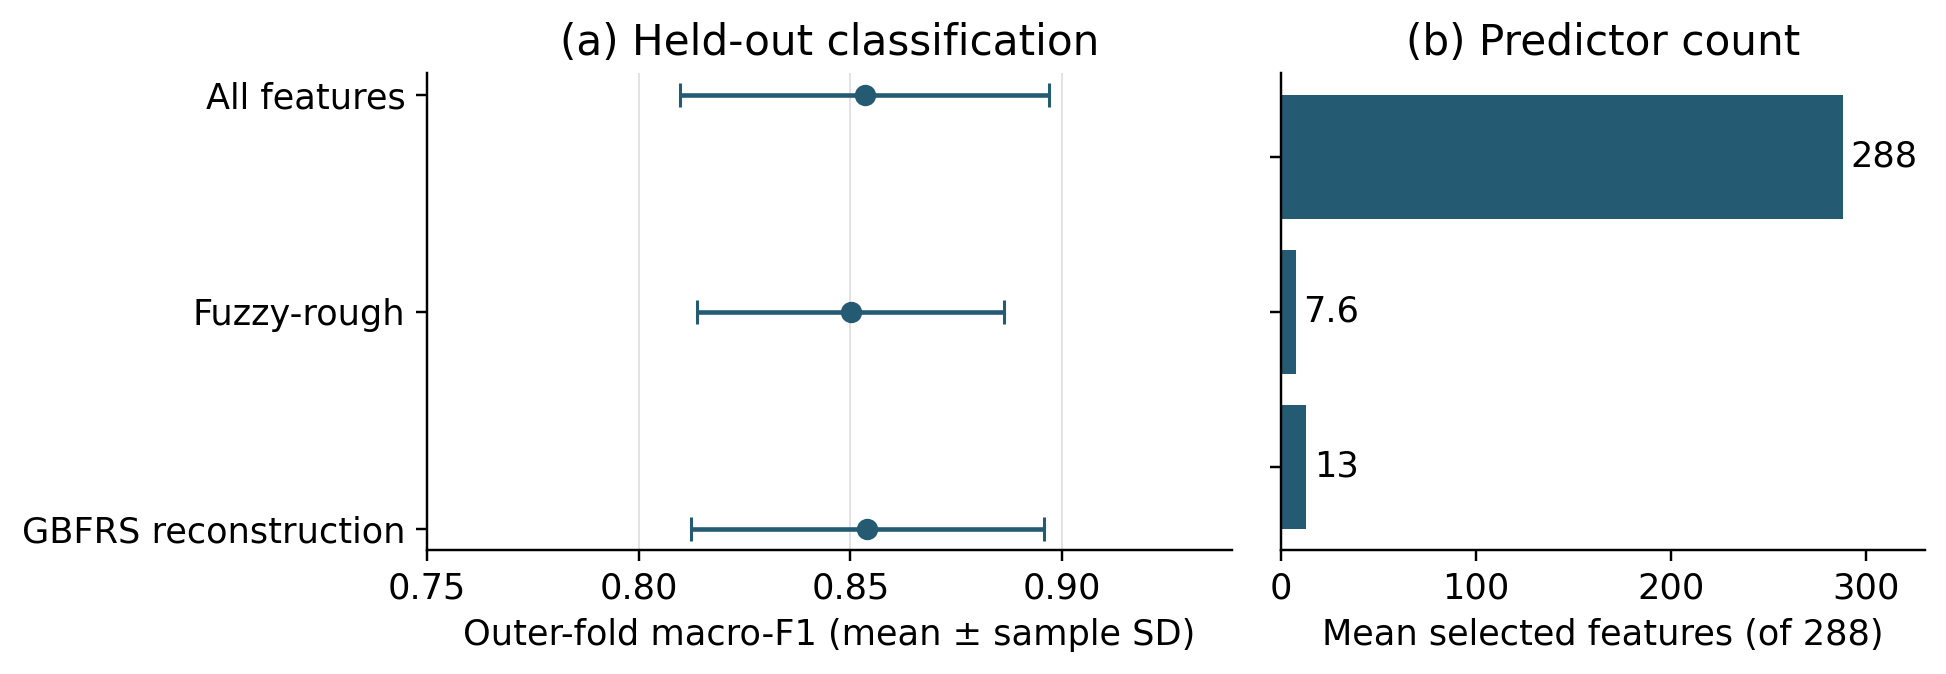
\includegraphics[width=\linewidth]{figures/performance-reduction.png}
\caption{Macro-F1 and number of classifier inputs on the fixed five-fold protocol. Error bars are sample SD across outer folds, not confidence intervals. Source: the complete 28 October 2026 rerun.}\label{fig:performance}
\end{figure}

Table~\ref{tab:clinical} reports the secondary class-specific summaries. Conventional fuzzy-rough selection has the highest observed mean malignant recall, whereas the granular-ball reconstruction has the highest observed mean benign specificity. These are descriptive differences under the shared default decision rule. They do not define clinically acceptable operating points, and no model has been selected using those outer-test trade-offs.
\begin{table}[htbp]\centering\small
\setlength{\tabcolsep}{4pt}\ClinicalTable
\caption{Secondary metrics, as outer-fold means and sample SDs. Malignant recall is sensitivity for class 1, and benign specificity is the true-negative rate for class 0.}\label{tab:clinical}
\end{table}

\subsection{Paired conditional uncertainty}
Table~\ref{tab:effects} and Figure~\ref{fig:effects} describe paired changes in \emph{pooled} OOF macro-F1. They intentionally use a different estimand from the mean-fold primary endpoint. The patient-level resampling unit reflects the one- or two-image grouping structure; treating images as independent bootstrap units would ignore that structure. The inferential scope remains conditional on the predictions produced by this particular nested evaluation.
\begin{table}[htbp]\centering\small
\setlength{\tabcolsep}{4pt}\resizebox{\linewidth}{!}{\EffectTable}
\caption{Differences in pooled OOF macro-F1 with conditional patient-stratified bootstrap intervals. These limits are descriptive and do not quantify uncertainty from repeating the full learning procedure.}\label{tab:effects}
\end{table}
\begin{figure}[htbp]\centering
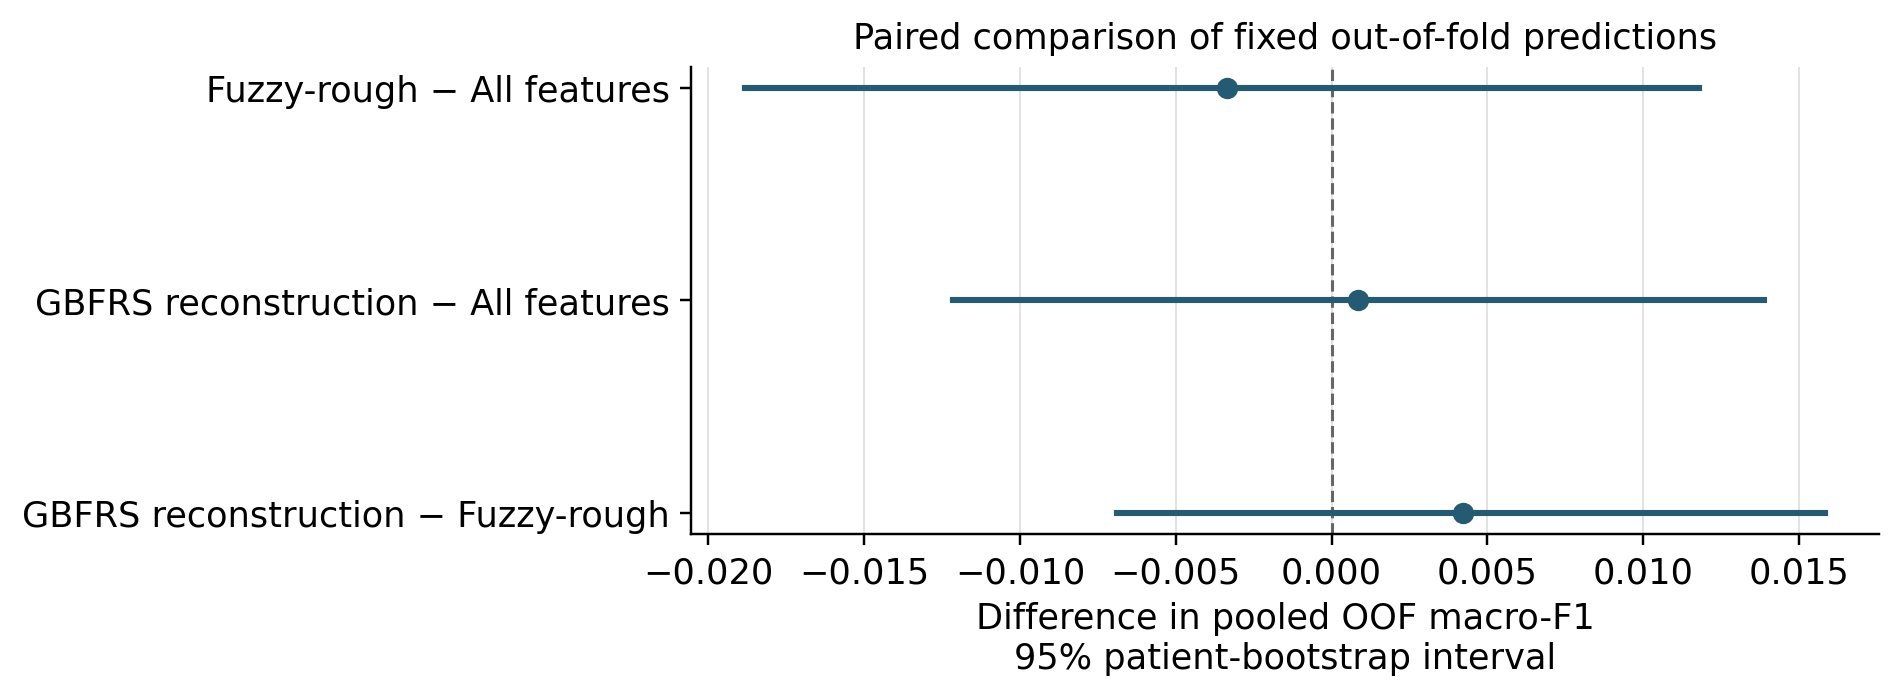
\includegraphics[width=\linewidth]{figures/paired-effects.png}
\caption{Paired differences in pooled macro-F1; the dashed line denotes zero. Intervals use the same 5,000 patient-cluster resamples for all methods. They must not be interpreted as an equivalence test.}\label{fig:effects}
\end{figure}

\subsection{Selection stability and measured computation}
Table~\ref{tab:stability} summarizes selection overlap, chance-adjusted stability and measured total wall time across five folds. The granular-ball reconstruction has higher observed named-set overlap than conventional fuzzy-rough selection in this experiment; this is a descriptive comparison of these five overlapping training sets, not evidence of general biological stability. Baseline overlap is one by construction, because it always includes every feature; this is not evidence that it discovers a better subset. The two selectors are evaluated on their own fold-specific sets, with no retrospective consensus subset substituted into the performance evaluation.
\begin{table}[htbp]\centering\small
\setlength{\tabcolsep}{5pt}\StabilityTable
\caption{Descriptive stability across five overlapping outer training sets and observed wall time. Methods ran sequentially with two SVM candidate workers and native threads limited to one. Desktop background activity was not controlled; times are machine dependent.}\label{tab:stability}
\end{table}
The selector timing field includes inner and outer selection, while the refit timing includes outer selection again. These overlapping fields are not added. The reported total uses the separately measured fold wall time, summed across folds. Feature selection itself can be costly even when the selected SVM input is small; a lower predictor count is not automatically a reduction in total training time or image-extraction cost.


\subsection{Broader baselines on the frozen ultrasound table}
Table~\ref{tab:bussecondary} combines the original primary results with the separately specified additional selectors and private author reference. ANOVA, mutual information and L1 logistic selection attain mean macro-F1 0.8391, 0.8469 and 0.8447, respectively. Their mean selected counts are 11.0, 9.0 and 30.8. The GBFRS reconstruction has the highest observed mean among these completed pipelines, but its 0.0006 advantage over the all-feature baseline is small. Without a confirmatory comparison, these point estimates do not establish superiority. The three additional baseline selectors also searched three times as many joint candidates. The unchanged private author selector also completes the BUS-BRA nested experiment, giving mean macro-F1 0.5034 (SD 0.0396) with 1.8 predictors. This substantial difference from the reconstruction is specific to the stated wrapper and downstream protocol; no source patch or outer-outcome tuning is applied.
\begin{table}[htbp]\centering\small
\setlength{\tabcolsep}{3pt}
\BusSecondaryTable
\caption{BUS-BRA primary pipelines and secondary baselines under the supplied patient-grouped folds. Accuracy and feature counts are outer-fold means. Additional selector settings are inner-tuned; fixed selectors have a smaller joint search budget.}\label{tab:bussecondary}
\end{table}

\subsection{Independent cytology benchmark and reference execution}
All seven WDBC pipelines complete five nested outer folds (Table~\ref{tab:wdbc}). The all-feature SVM gives macro-F1 0.9772 with 30 predictors; ANOVA gives the same rounded mean with 20 predictors. Conventional fuzzy-rough selection gives 0.9455 with 5.6 predictors and the reconstruction gives 0.9603 with 4.8. Thus the apparent performance--compactness relationship on BUS-BRA does not imply a general advantage across datasets.

The unchanged author selector gives mean WDBC macro-F1 0.8366 with 2.8 predictors, compared with 0.9603 and 4.8 for the reconstruction. This difference is specific to the declared wrapper, seed, purity, folds and SVM setting. Together with the synthetic dependency fixture, it shows that the two programs are not interchangeable in this study. It does not establish that the reconstruction is the definitive GBFRS algorithm or that the authors' published results are wrong. The public audit records the exact source hash, and the private outputs retain each nested search.
\begin{table}[htbp]\centering\small
\setlength{\tabcolsep}{3pt}
\WdbcTable
\caption{Secondary WDBC cytology benchmark: five case-level stratified outer folds, separately trained pipelines and training-only inner selection. This is not an external ultrasound cohort or a patient-disjointness claim based on verified WDBC patient identifiers.}\label{tab:wdbc}
\end{table}


\subsection{Training-label corruption}\label{sec:noiseresults}
All six prespecified corruption runs complete. At nominal 10\% corruption, macro-F1 is 0.8299 for the all-feature SVM, 0.7898 for conventional fuzzy-rough selection and 0.8405 for the reconstruction. At nominal 20\%, the corresponding values are 0.8094, 0.7548 and 0.8181. Table~\ref{tab:noise} includes the clean references; Figure~\ref{fig:noise} shows the change across nominal rates. The reconstruction has higher observed means than the other two pipelines in these corruption draws, while all three deteriorate relative to their clean runs. This is not a general noise-robustness guarantee: patient-group counts are rounded within class, only one corruption draw is used per fold/rate, and no multiplicity-adjusted confirmatory tests are performed.
\begin{table}[htbp]\centering\small
\setlength{\tabcolsep}{3pt}\NoiseTable
\caption{Training-patient label corruption on BUS-BRA. Rates are nominal; test labels remain clean. Values are five outer-fold means and sample SDs. Settings are specified before these outcomes, with 32 SVM candidates per setting.}\label{tab:noise}
\end{table}
\begin{figure}[htbp]\centering
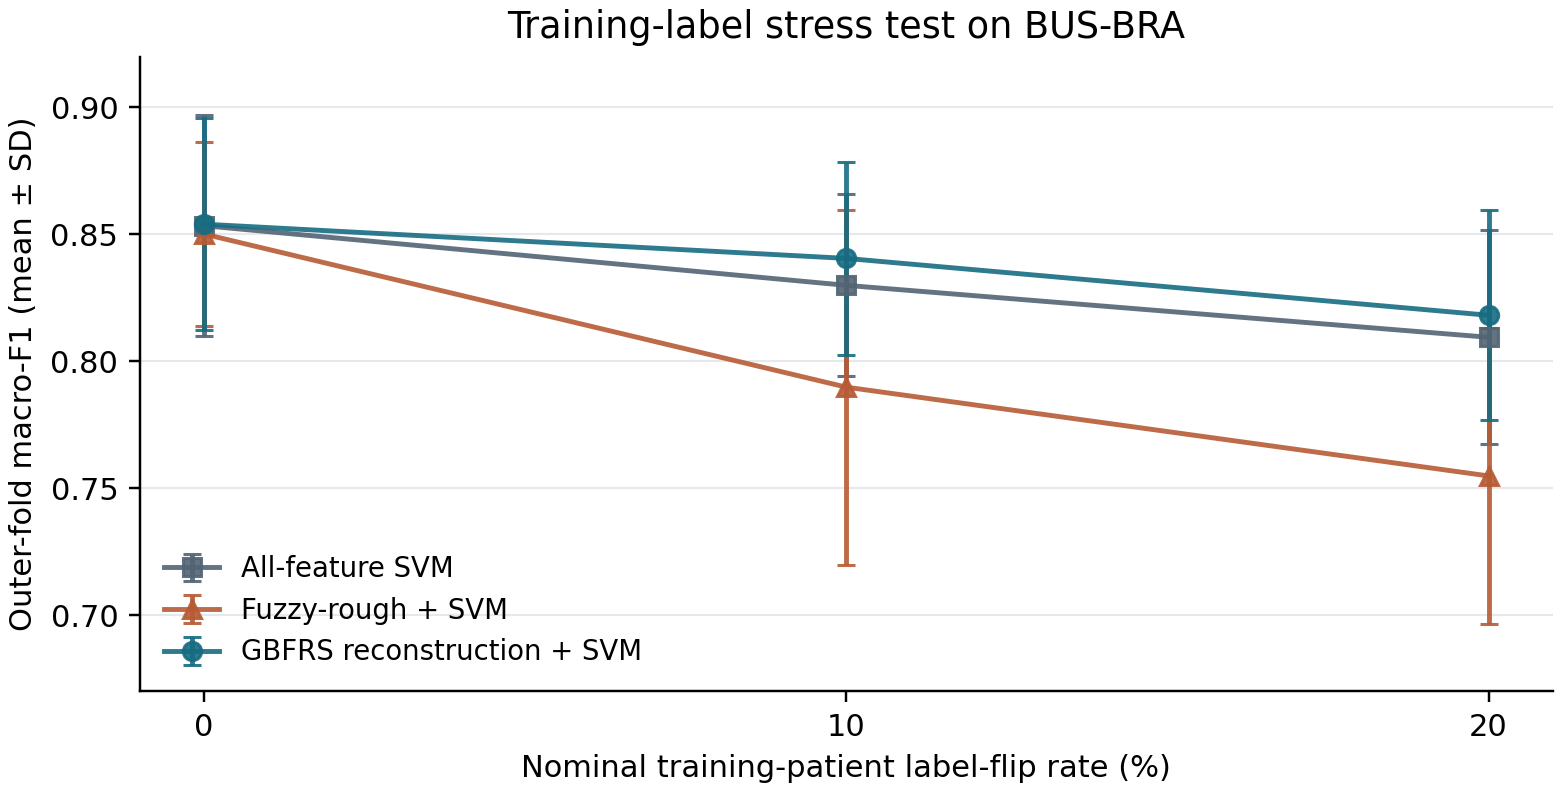
\includegraphics[width=0.9\linewidth]{figures/label-noise.png}
\caption{Descriptive label-corruption stress test. Error bars are fold SDs, not confidence intervals. A common corrupted-patient draw is used across methods within each outer fold and rate.}\label{fig:noise}
\end{figure}

\subsection{Sensitivity and isolated dependency-expression effect}\label{sec:ablationresults}
The four purity/seed sensitivity runs complete with macro-F1 between 0.8504 and 0.8537; their primary reference is 0.8540 (Table~\ref{tab:sensitivity}). Mean predictor counts range from 12.8 to 14.8, compared with 13.0 in the reference. The small observed range is limited to these particular settings and folds and does not demonstrate invariance to initialization or purity.

By contrast, changing only the dependency expression to Equation~\ref{eq:alternative} produces macro-F1 0.5051 (SD 0.0393), selecting 1.8 predictors on average. This isolates a material criterion effect within the reconstruction, beyond the earlier whole-program comparison. It does not prove that every difference in the full author program is caused by that expression, or identify which implementation is the definitive journal method. The result supports explicit equation/code auditing when interpreting a GBFRS reproduction.
\begin{table}[htbp]\centering\small
\setlength{\tabcolsep}{3pt}\SensitivityTable
\caption{Separate nested GBFRS sensitivity runs and a controlled dependency ablation. ``Own'' uses Equation~\ref{eq:gb}; the alternative uses Equation~\ref{eq:alternative} with the same reconstruction ball-construction procedure. No setting is selected using outer outcomes.}\label{tab:sensitivity}
\end{table}

\subsection{Results on the independent ultrasound cohort}\label{sec:externalresults}
All six separately retrained BrEaST pipelines complete their nested evaluation (Table~\ref{tab:external}). ANOVA gives macro-F1 0.7296 with 18.0 predictors, and L1 selection gives 0.7272 with 9.6. The all-feature SVM gives 0.6886 with 102 predictors, conventional fuzzy-rough selection gives 0.6737 with 5.8, and reconstructed GBFRS gives 0.6700 with 12.2. Thus a favorable point comparison for compact GBFRS inputs on BUS-BRA does not extend uniformly to this ultrasound cohort. Since extraction basis, acquisition population and available predictors differ, the numerical change is not an isolated estimate of model-transfer degradation. This cohort evaluates independently retrained methods; it is not a held-out test of the previously fitted BUS-BRA classifier.
\begin{table}[htbp]\centering\small
\setlength{\tabcolsep}{3pt}\ExternalTable
\caption{BrEaST: 252 lesion cases from distinct patients, 102 separately extracted original-image features and five stratified outer folds. Values are fold means and sample SDs. Three-setting selectors search 96 joint configurations, fixed selectors 32. No source images, patient rows or predictions are publicly exported.}\label{tab:external}
\end{table}

\section{Discussion and limitations}
The principal observation is a trade-off between a large reduction in classifier inputs and close observed performance under one fixed evaluation. This is useful as an empirical result even without a consistent accuracy improvement. It encourages examination of compact subsets, while preserving the distinction between an observed similarity and a statistically supported equivalence claim.

Several limitations restrict the scope. First, the primary comparison uses one prepared BUS-BRA dataset and one fixed five-fold design. The independent BrEaST cohort adds ultrasound evidence with a public extraction protocol, but its models are retrained on a different 102-feature basis. We still lack external testing of a frozen BUS-BRA-trained model, prospective evaluation and the original upstream extraction configuration. WDBC changes both modality and predictors and supplies an additional method benchmark rather than an ultrasound transportability test. The outer folds have overlapping training sets, and the supplementary conditional bootstrap does not remove the uncertainty associated with that overlap. Re-executing the same protocol is a software reproducibility check, not an additional independent scientific replication.

Second, three primary pipelines are supplemented by ANOVA, mutual-information and L1 logistic selection, but the study does not cover the broader range of embedded selectors, radiomics workflows or deep-learning systems. The secondary baselines have a larger joint search budget, and WDBC results do not support a universal advantage for either fuzzy-rough pipeline. The added patient-label stress tests use one synthetic corruption draw per fold/rate. They do not evaluate image noise, repeated corruption seeds or the full robustness claims of the source GBFRS paper. The primary purity threshold remains fixed rather than inner-tuned. The new purity/seed runs are separate sensitivity analyses and do not replace that primary setting based on outer scores.

Third, the granular-ball implementation is a qualified reconstruction. Differences between the accessible equations and inspected code required explicit choices. Reporting those choices makes this particular experiment inspectable; it does not settle which implementation should be regarded as the definitive journal algorithm. The pinned unchanged author selector has now been executed privately on both BUS-BRA and WDBC and compared with the reconstruction, and a synthetic criterion discrepancy is demonstrated. The fixed-construction criterion ablation further localizes a large implementation effect in this experimental setting. These checks clarify non-equivalence without establishing an exact replication of the original publication. Licensing and classifier/protocol harmonization still matter for a distributable reference benchmark.

Fourth, this is an image-level classification task with patient-grouped splitting, not a patient-level diagnostic endpoint. Lesion masks are assumed available. Calibration, reader comparison, downstream decisions and clinical net benefit are not evaluated. Device and demographic subgroup analyses are not available from the permitted predictor table, so transportability and subgroup fairness remain unassessed. The absence of physical pixel spacing also limits interpretation of geometric radiomic quantities.

Fifth, feature stability is measured on named columns with known redundancies. Selecting alternative correlated or numerically equivalent columns can produce low named-set overlap. Stability should therefore not be treated as direct evidence for or against a reproducible biological mechanism. The study does not replace unstable names with new engineered features, since that would change the frozen candidate matrix.

Finally, the original protocol was established in the team handoff, not prospectively registered in a public registry. The uncertainty and stability reporting were added during manuscript preparation after the initial results had been seen. They are explicitly secondary descriptive analyses. The primary rerun keeps the model definitions, source folds, SVM grid and selector settings unchanged. The additional methods, WDBC benchmark, robustness studies and independent ultrasound cohort follow separate specifications written after seeing earlier outcomes but before inspecting their own outcomes; they remain exploratory descriptive evidence.

\section{Reproducibility and research statements}
\subsection{Code and execution}
The public repository is \href{https://github.com/naazzarov/busbra-ultrasound-classification}{\texttt{naazzarov/busbra-ultrasound-classification}}. It includes method definitions, the frozen evaluation contract, dependency lockfile, test suite, aggregate results, manuscript source and figure-generation code. The primary rerun uses Python 3.12, NumPy 2.2.6, pandas 2.3.3, SciPy 1.15.3, scikit-learn 1.6.1, joblib 1.5.3 and threadpoolctl 3.6.0. Exact platform information is recorded in the primary aggregate artifact. The secondary protocol and runner are separate, with a validator checking observation/label/fold alignment, recomputed fold metrics, candidate counts and exported source checksums before aggregate publication. Matplotlib 3.10.8 generates figures in a separate environment and is not part of model training.

The \texttt{run-all} command executes the complete frozen evaluation sequentially for all methods. A run manifest records completion or failure without overwriting previous runs. Each private submission contains the original five CSV/JSON outputs, full inner-search records, selected names, dependency histories, source checksums and runnable source. The comparison checker verifies paired observation/group/fold/label alignment. Software tests separately audit training-only fitting boundaries; output validation alone cannot prove absence of methodological leakage.

\subsection{Data availability and ethics scope}
The original anonymized BUS-BRA images are distributed by their creators through Zenodo \cite{zenodo}. We do not redistribute images, the private prepared table, group identifiers, individual predictions or fitted model artifacts. The public release contains aggregate measurements and derived figures. WDBC is obtained through the bundled scikit-learn dataset; its source is credited to UCI under CC BY 4.0, and no case-level copy is included in this release. Reproduction of the exact downstream experiment requires authorized access to the unchanged prepared table; access to the original images alone does not fully specify that table without the upstream extraction environment.

The public BrEaST images, lesion masks and clinical labels are distributed through TCIA under CC BY 4.0 \cite{breast}. The experiment records source checksums and publishes extraction code and aggregate results; source data, extracted case-level tables and predictions are not included in this repository.

This work is a secondary computational analysis. No new patient recruitment or data collection is reported. The source dataset's ethical and collection context should be read in its original publication. This manuscript does not assert an independent ethics exemption, institutional approval or clinical validation that has not been documented.

\subsection{Acknowledgments and assistance}
The authors acknowledge Luo Chuan. AI tools assisted with implementation, analysis and drafting; the authors are responsible for the manuscript.

\section{Conclusion}
Under a frozen patient-grouped nested protocol, conventional fuzzy-rough selection and a qualified granular-ball reconstruction reduce the SVM predictor count substantially while yielding macro-F1 point estimates close to the all-feature baseline. The result supports further study of compact radiomic classifier inputs on BUS-BRA. It does not establish clinical performance, statistical equivalence or a general advantage of granular-ball selection. The broader comparator set and separate cytology results bound this observation: fuzzy-rough selection is not uniformly preferable, and the private author selector is not numerically interchangeable with the reconstruction. The independent ultrasound cohort does not support a universal GBFRS advantage, while the controlled criterion ablation demonstrates a substantial implementation-dependent effect. Frozen-model external testing and human author review remain necessary before stronger claims or submission.

\begin{thebibliography}{99}
\bibitem{busbra} W. G\'omez-Flores, M. J. Gregorio-Calas, and W. Coelho de Albuquerque Pereira. BUS-BRA: A breast ultrasound dataset for assessing computer-aided diagnosis systems. \emph{Medical Physics}, 51:3110--3123, 2024. \url{https://doi.org/10.1002/mp.16812}.
\bibitem{zenodo} W. G\'omez-Flores, M. J. Gregorio-Calas, and W. Coelho de Albuquerque Pereira. BUS-BRA dataset, version 1.0. Zenodo. \url{https://doi.org/10.5281/zenodo.8231412}.
\bibitem{pyradiomics} J. J. M. van Griethuysen et al. Computational radiomics system to decode the radiographic phenotype. \emph{Cancer Research}, 77(21):e104--e107, 2017. \url{https://doi.org/10.1158/0008-5472.CAN-17-0339}.
\bibitem{jensen} R. Jensen and Q. Shen. New approaches to fuzzy-rough feature selection. \emph{IEEE Transactions on Fuzzy Systems}, 17(4):824--838, 2009. \url{https://doi.org/10.1109/TFUZZ.2008.924209}.
\bibitem{xia} S. Xia, X. Lian, B. Sang, G. Wang, and X. Gao. GBFRS: Robust fuzzy rough sets via granular-ball computing. arXiv:2501.18413v1, 2025. \url{https://arxiv.org/abs/2501.18413}. Our implemented target is this accessible preprint; the later journal record is \url{https://doi.org/10.1109/TNNLS.2026.3681370}.
\bibitem{varma} S. Varma and R. Simon. Bias in error estimation when using cross-validation for model selection. \emph{BMC Bioinformatics}, 7:91, 2006. \url{https://doi.org/10.1186/1471-2105-7-91}.
\bibitem{svm} C. Cortes and V. Vapnik. Support-vector networks. \emph{Machine Learning}, 20:273--297, 1995. \url{https://doi.org/10.1007/BF00994018}.
\bibitem{sklearn} F. Pedregosa et al. Scikit-learn: Machine learning in Python. \emph{Journal of Machine Learning Research}, 12:2825--2830, 2011. \url{https://jmlr.org/papers/v12/pedregosa11a.html}.
\bibitem{nogueira} S. Nogueira, K. Sechidis, and G. Brown. On the stability of feature selection algorithms. \emph{Journal of Machine Learning Research}, 18(174):1--54, 2018. \url{https://jmlr.org/papers/v18/17-514.html}.
\bibitem{wdbc} W. Wolberg, O. Mangasarian, N. Street, and W. Street. Breast Cancer Wisconsin (Diagnostic) [Dataset]. UCI Machine Learning Repository, 1993. \url{https://doi.org/10.24432/C5DW2B}. CC BY 4.0.
\bibitem{authorcode} X. Lian. GBFRS author-linked code archive. GitHub, inspected commit \texttt{0382e0899b0dc5529c89d1b9a11da198464d49ad}. \url{https://github.com/lianxiaoyu724/GBFRS}.
\bibitem{tripod} G. S. Collins et al. TRIPOD+AI statement: Updated guidance for reporting clinical prediction models that use regression or machine learning methods. \emph{BMJ}, 385:e078378, 2024. \url{https://doi.org/10.1136/bmj-2023-078378}.

\bibitem{skinnytrees} S. Ibrahim, K. Behdin, and R. Mazumder. End-to-end feature selection approach for learning Skinny Trees. In \emph{Proceedings of the 27th International Conference on Artificial Intelligence and Statistics (AISTATS)}, PMLR 238:2863--2871, 2024. \url{https://proceedings.mlr.press/v238/ibrahim24a.html}.
\bibitem{localleakage} H. Oosterhuis, L. Lyu, and A. Anand. Local feature selection without label or feature leakage for interpretable machine learning predictions. In \emph{Proceedings of the 41st International Conference on Machine Learning (ICML)}, PMLR 235:38740--38761, 2024. \url{https://proceedings.mlr.press/v235/oosterhuis24a.html}.
\bibitem{robustselection} M. Swaroop, T. Krishnamurti, and B. Wilder. Distributionally robust feature selection. In \emph{Advances in Neural Information Processing Systems}, 38, NeurIPS, 2025. \url{https://doi.org/10.52202/085713-2117}.
\bibitem{adaptation} Y. Duan et al. ADAptation: Reconstruction-based unsupervised active learning for breast ultrasound diagnosis. In \emph{Medical Image Computing and Computer Assisted Intervention -- MICCAI 2025}, LNCS 15975:35--45, 2025. \url{https://doi.org/10.1007/978-3-032-05325-1_4}.
\bibitem{samask} P. Xu et al. SAMASK-CLTR: A spatial-aware mask guided learning model for benign and malignant tumor classification in ABUS. In \emph{Medical Image Computing and Computer Assisted Intervention -- MICCAI 2025}, LNCS 15960:567--577, 2025. \url{https://doi.org/10.1007/978-3-032-04927-8_54}.
\bibitem{breast} A. Paw\l{}owska et al. Curated benchmark dataset for ultrasound based breast lesion analysis. \emph{Scientific Data}, 11:148, 2024. \url{https://doi.org/10.1038/s41597-024-02984-z}. BrEaST (BREAST-LESIONS-USG) data release, TCIA, CC BY 4.0: \url{https://doi.org/10.7937/9WKK-Q141}.
\end{thebibliography}
\end{document}
